% Assignment 3 - ChannelNet (Deep Learning-Based Channel Estimation)
\documentclass[a4paper,10pt]{article}

\newenvironment{packed_enum}{
\begin{enumerate}
  \setlength{\itemsep}{1.5pt}
  \setlength{\parskip}{0pt}
  \setlength{\parsep}{0pt}
}{\end{enumerate}}

\usepackage{graphicx}
\usepackage{fancyhdr}
\usepackage{geometry}
\usepackage{amsmath}
\usepackage{float}
\usepackage{pifont}
\usepackage{indentfirst}
\usepackage[T1]{fontenc}
\usepackage{xcolor}
\usepackage[colorlinks=true, linkcolor=blue, urlcolor=blue, citecolor=blue]{hyperref}
\usepackage{listings}
\usepackage{tcolorbox}
\tcbuselibrary{listings,breakable}
\usepackage{subcaption}
\usepackage[export]{adjustbox}
\usepackage{amsfonts}
\usepackage{amssymb}
\usepackage{booktabs}
\usepackage{csquotes}

\definecolor{mywhite}{HTML}{f3f4f7}
\definecolor{mygreen}{HTML}{449944}
\definecolor{iiitbblue}{HTML}{01519a}

\lstdefinestyle{mystyle}{
    commentstyle=\color{mygreen},
    keywordstyle=\color{blue},
    stringstyle=\color{purple},
    basicstyle=\ttfamily\small,
    breakatwhitespace=false,
    breaklines=true,
    captionpos=t,
    frame=lines,
    rulecolor=\color{black},
    keepspaces=true,
    numbers=left,
    numbersep=5pt,
    showspaces=false,
    showstringspaces=false,
    showtabs=false,
    tabsize=2
}
\lstset{style=mystyle}

\lstdefinestyle{mypython}{
    language=Python,
    backgroundcolor=\color{white},
    commentstyle=\color{mygreen},
    keywordstyle=\color{blue}\bfseries,
    stringstyle=\color{purple},
    basicstyle=\ttfamily\small,
    breakatwhitespace=false,
    breaklines=true,
    captionpos=t,
    frame=lines,
    rulecolor=\color{black},
    keepspaces=true,
    numbers=left,
    numbersep=5pt,
    showspaces=false,
    showstringspaces=false,
    showtabs=false,
    tabsize=4,
    morekeywords={as, lambda, with, yield, async, await, None, True, False},
    morecomment=[s]{"""}{"""},
    morecomment=[s]{'''}{'''},
    literate=
     {á}{{\'a}}1 {é}{{\'e}}1 {í}{{\'i}}1 {ó}{{\'o}}1 {ú}{{\'u}}1
}

\lstdefinestyle{mymatlab}{
    language=Matlab,
    backgroundcolor=\color{white},
    commentstyle=\color{mygreen},
    keywordstyle=\color{blue}\bfseries,
    stringstyle=\color{purple},
    basicstyle=\ttfamily\small,
    breaklines=true,
    captionpos=t,
    frame=lines,
    rulecolor=\color{black},
    keepspaces=true,
    numbers=left,
    numbersep=5pt,
    showstringspaces=false,
    tabsize=4
}

\lstdefinestyle{terminal}{
    backgroundcolor=\color{black},
    basicstyle=\ttfamily\small\color{white},
    breaklines=true,
    prebreak=\raisebox{0ex}[0ex][0ex]{\ensuremath{\hookleftarrow}},
    postbreak=\raisebox{0ex}[0ex][0ex]{\ensuremath{\hookrightarrow\space}},
    frame=none,
}

\geometry{a4paper, total={170mm,257mm}, left=20mm, right= 20mm, top=20mm, bottom = 20mm, headheight=40pt}

\graphicspath{{Images/}}

\pagestyle{fancy}
\fancyhf{}
\renewcommand{\headrulewidth}{0pt}
\rfoot{\thepage}

\title{\vspace{-2 cm}\Huge\textbf{Assignment 3} \\
    \vspace{0.5cm}\normalsize COM 837 ML for Wireless Communication \\
    \normalsize Deep Learning-Based Channel Estimation (ChannelNet) \\
    \normalsize Hardhik Dhavala (IMT2023579) \\
    }
\date{\vspace{-1cm}\today}

\begin{document}

\maketitle
\thispagestyle{fancy}
\vspace{-0.4cm}

% ============================================================
\section{Overview}
% ============================================================
I reproduce \textit{ChannelNet} \cite{soltani2019}. It treats the $72\times14$ time--frequency channel as an image and the pilot estimate as a low-resolution, noisy version of it. An SRCNN \cite{dong2016} super-resolution stage and a DnCNN \cite{zhang2017} restoration stage then recover the full channel. I compare it with LS + 2-D interpolation and with MMSE, on VehA and SUI5 channels, across SNR and pilot density. Channels were generated in MATLAB R2025b with the supplied Vienna 5G Link-Level Simulator \cite{vienna}. Everything else ran in Python/PyTorch on Kaggle ($2\times$ NVIDIA T4, $\approx$3~h for the whole pipeline). The code is modular, with separate training (\texttt{train.py}) and testing (\texttt{test.py}) scripts, one configuration file (\texttt{src/config.py}) and saved checkpoints. The README gives the exact steps, and the code is also in my course repository \cite{github}.

% ============================================================
\section{Dataset Generation (Task 1)}
% ============================================================
\textbf{System model.} The SISO-OFDM subframe has $N_S=72$ subcarriers (15~kHz, LTE 1.4~MHz) and $N_D=14$ symbols. Each resource element follows paper Eq.~(1):
\begin{equation}
    Y[i,k] = H[i,k]\,X[i,k] + Z[i,k], \qquad Z\sim\mathcal{CN}(0,\sigma^2),
    \label{eq:sysmodel}
\end{equation}
with unit-power pilots and $\mathbb{E}|H|^2=1$, so $\text{SNR}=1/\sigma^2$.

\textbf{Channels.} I used the simulator's \texttt{FastFading} class (\texttt{matlab/gen\_channels.m}) at 3.84~MHz (256-point FFT). The transfer function is taken at the centre of each OFDM symbol and the 72 active subcarriers are kept. Following the paper, the carrier is 2.1~GHz and the speed 50~km/h, giving a maximum Doppler of 97~Hz (Jakes, 100 paths, independent subframes). \textbf{VehA} is built into the simulator (RMS delay spread 0.38~$\mu$s). \textbf{SUI5} is not, so I passed it as a user-defined power-delay profile: 0/4/10~$\mu$s and 0/$-$5/$-$10~dB (RMS delay spread 2.80~$\mu$s). I generated 40\,000 channels per model (seeds 1, 2) and split them 32\,000/4\,000/4\,000 into train/val/test with a fixed permutation (seed 0), as in the paper. Each complex channel becomes two real images, its real and imaginary parts (Fig.~\ref{fig:gt}). Both go through the same network and are normalised by the target standard deviation ($\approx0.707$). With this scale, the normalised loss equals the complex MSE $\mathbb{E}|\hat H-H|^2$.

\textbf{Pilots.} I use lattice (diamond) patterns (Fig.~\ref{fig:gt}c). The main pattern has \textbf{48 pilots}, matching LTE CRS port 0: symbols 0, 4, 7, 11, every 6th subcarrier, shifted by 3 subcarriers between pilot symbols. The pilot study adds 24, 36 and 72 pilots.

\begin{figure}[H]
    \centering
    \begin{subfigure}{0.33\textwidth}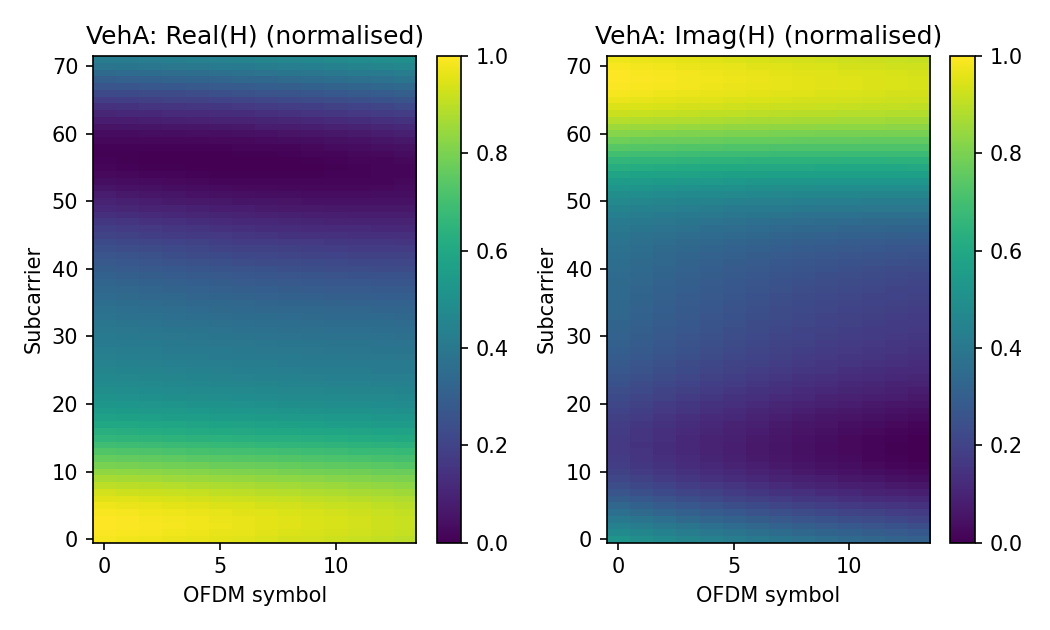
\includegraphics[width=\textwidth]{fig_groundtruth_VehA.png}\caption{VehA}\end{subfigure}\hfill
    \begin{subfigure}{0.33\textwidth}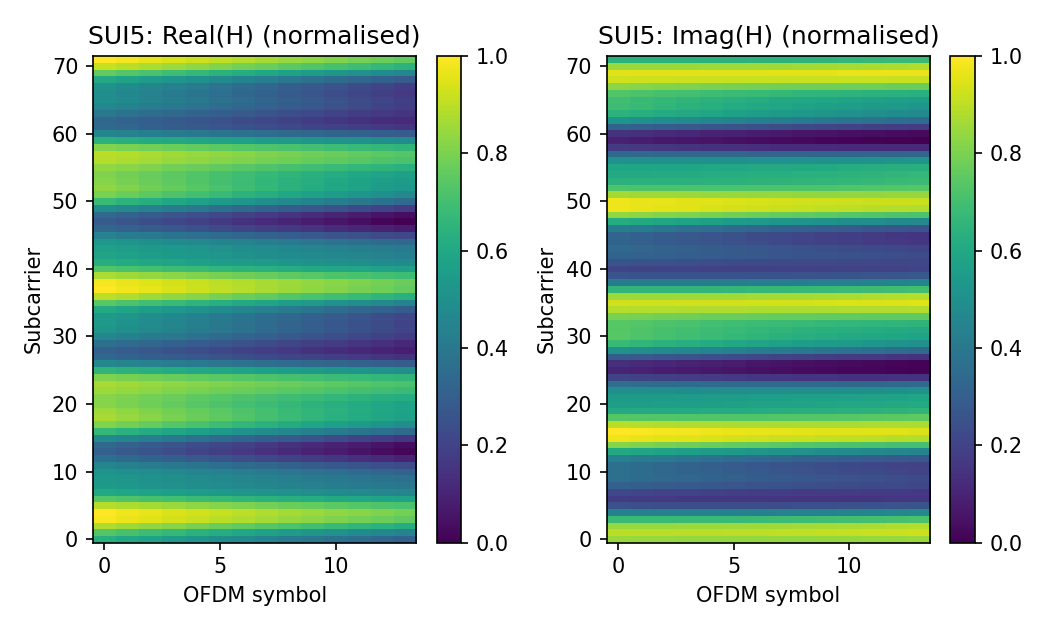
\includegraphics[width=\textwidth]{fig_groundtruth_SUI5.png}\caption{SUI5}\end{subfigure}\hfill
    \begin{subfigure}{0.32\textwidth}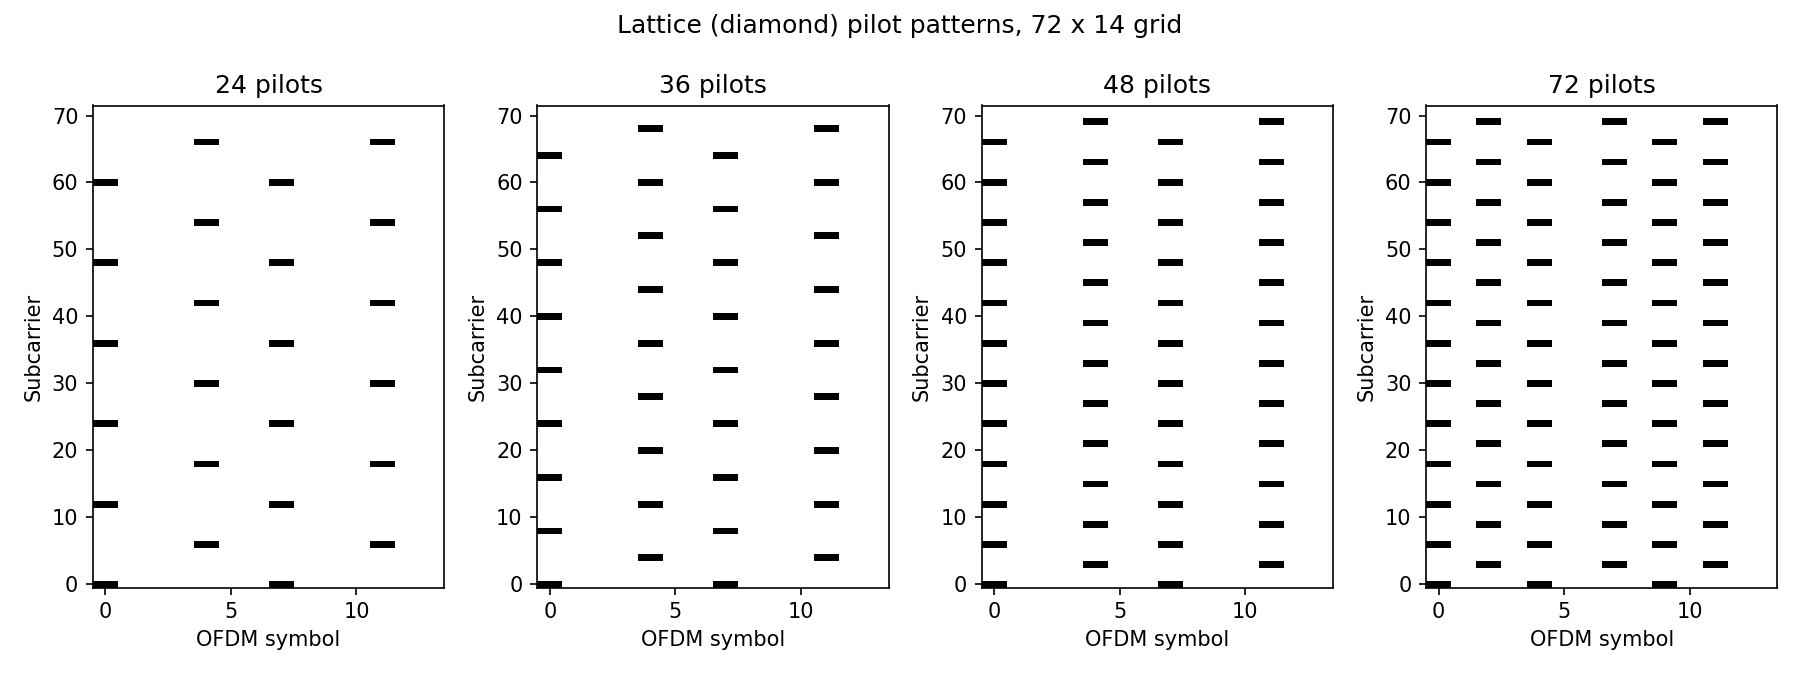
\includegraphics[width=\textwidth]{fig_pilot_patterns.png}\caption{Pilot patterns (24/36/48/72)}\end{subfigure}
    \caption{Ground-truth real/imaginary channel images (normalised) and lattice pilot patterns}
    \label{fig:gt}
\end{figure}
VehA is smooth. SUI5 shows stripes, because its 10~$\mu$s path makes the response repeat every 100~kHz, which is about 7 subcarriers. With pilots on every 6th subcarrier, SUI5 is hard to reconstruct.

% ============================================================
\section{Conventional Estimation (Task 2)}
% ============================================================
\textbf{LS + 2-D interpolation.} At pilot positions, $\hat h_{LS}=y_p/x_p=h_p+z_p/x_p$ (paper Eq.~(2)). The pilot estimates are spread over the grid with 2-D linear (Delaunay) interpolation, plus nearest-neighbour filling outside the pilots' convex hull. This interpolation is linear in the pilot values, so I implemented it exactly as a fixed matrix $W\in\mathbb{R}^{1008\times N_p}$, giving $\text{vec}(\hat H_{LS})=W\hat h_{LS}$. The same image is the SRCNN input.

\textbf{MMSE.} With unit pilots, paper Eqs.~(3)--(5) (see also \cite{edfors1998}) give
\begin{equation}
    \hat h_{MMSE}=A\hat h_{LS},\qquad A=R_{hp}\left(R_{pp}+\sigma^2 I\right)^{-1}.
\end{equation}
\textit{Ideal MMSE} takes $R=\mathbb{E}[hh^H]$ from the 32\,000 true training channels; this is a benchmark no real receiver can reach. \textit{Estimated MMSE} takes $R$ from only 1\,000 noisy LS-interpolated frames, after subtracting the known noise term $\sigma^2WW^T$; this is the practical counterpart of the paper's approximated MMSE. The results are in Table~\ref{tab:results}. For SUI5, LS and estimated MMSE hit an \textbf{error floor of $\approx$0.13}. Interpolation cannot follow the fast frequency variation, and estimated MMSE learns its statistics from the same smoothed data.

% ============================================================
\section{ChannelNet and Training (Tasks 3, 4, 5)}
% ============================================================
\begin{table}[H]
\centering
\caption{ChannelNet architecture (`same' padding keeps $72\times14$)}
\label{tab:arch}
\small
\begin{tabular}{llr}
\toprule
\textbf{Stage} & \textbf{Layers} & \textbf{Params} \\
\midrule
SRCNN (SR) & Conv $9\times9$,64+ReLU $\rightarrow$ Conv $1\times1$,32+ReLU $\rightarrow$ Conv $5\times5$,1 & 8\,129 \\
DnCNN (DN) & Conv $3\times3$,64+ReLU $\rightarrow$ 18$\times$[Conv $3\times3$,64+BN+ReLU] $\rightarrow$ Conv $3\times3$,1 (residual) & 667\,073 \\
\bottomrule
\end{tabular}
\end{table}
\vspace{-0.2cm}
\textbf{Two-stage training (paper Sec.~III-C).} Stage~1 trains SRCNN to minimise $C_1=\text{mean}\|f_S(X)-H\|^2$, where $X$ is the noisy interpolated LS image. Stage~2 \emph{freezes} SRCNN, computes $Z=f_S(X)$, and trains DnCNN to minimise $C_2=\text{mean}\|f_R(Z)-H\|^2$. DnCNN uses residual learning: it predicts the remaining noise $\hat n$, and the output is $Z-\hat n$. I trained separate networks per channel model and per SNR: 12~dB (``deep low-SNR'') and 22~dB (``deep high-SNR''). For the pilot study, I also trained networks for 24/36/72 pilots at 12~dB, giving 20 checkpoints in total.

\begin{table}[H]
\centering
\caption{Training settings}
\label{tab:settings}
\small
\begin{tabular}{lp{12.3cm}}
\toprule
Optimiser & Adam, lr $10^{-3}$, batch 128 (paper); ReduceLROnPlateau ($\times0.5$); early stopping (patience 10), best-validation weights kept \\
Epochs & SRCNN max 100 (used 99--100); DnCNN max 40 for 48 pilots (used 33/39/40/40), max 20 for the pilot sweep \\
Data / noise & 64\,000/8\,000/8\,000 real+imag images; one fixed AWGN realisation per frame at the training SNR; test noise identical for all methods \\
Reproducibility & Python/NumPy/PyTorch seeds, deterministic cuDNN; split seed 0, noise base seed 1234; all settings in \texttt{src/config.py} \\
Hardware & Kaggle $2\times$T4, mixed precision; SRCNN $\approx$3~s/epoch, DnCNN $\approx$25~s/epoch \\
\bottomrule
\end{tabular}
\end{table}

\begin{figure}[H]
    \centering
    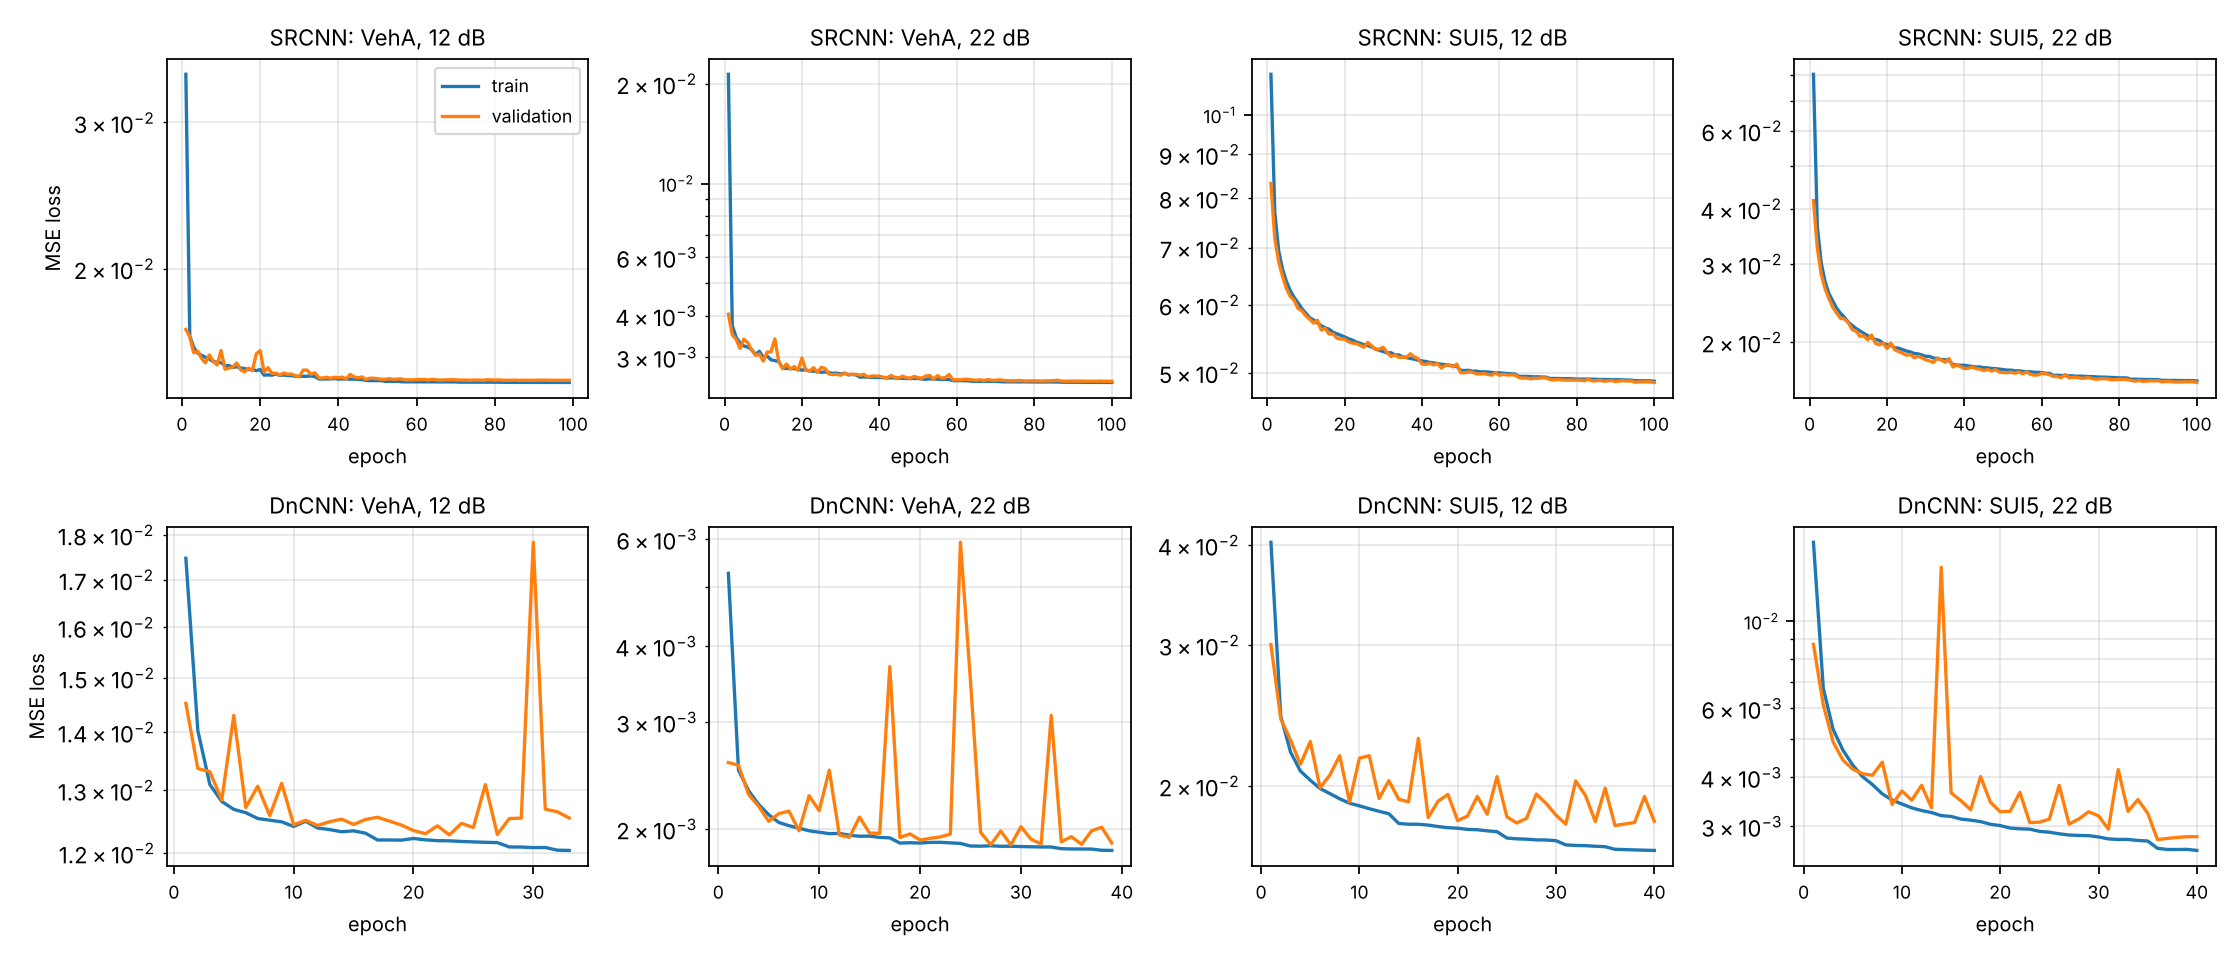
\includegraphics[width=0.93\textwidth]{fig_losses.png}
    \caption{Training/validation loss vs.\ epoch: SR stage (top) and DN stage (bottom), 48 pilots}
    \label{fig:losses}
\end{figure}
The training and validation curves almost overlap in every case (Fig.~\ref{fig:losses}), so the model does not overfit. Table~\ref{tab:ablation} shows how much each stage contributes. The DN stage matters most for SUI5, where it cuts the error 2.7--5.8$\times$.

\begin{table}[H]
\centering
\caption{Best validation MSE after each stage (48 pilots, at the training SNR)}
\label{tab:ablation}
\small
\begin{tabular}{lcccc}
\toprule
\textbf{Network} & \textbf{LS input} & \textbf{After SRCNN} & \textbf{After DnCNN} & \textbf{DnCNN gain} \\
\midrule
VehA, 12 / 22~dB & 4.06e-2 / 5.57e-3 & 1.47e-2 / 2.54e-3 & 1.23e-2 / 1.88e-3 & 1.2$\times$ / 1.3$\times$ \\
SUI5, 12 / 22~dB & 1.68e-1 / 1.33e-1 & 4.87e-2 / 1.62e-2 & 1.78e-2 / 2.77e-3 & 2.7$\times$ / 5.8$\times$ \\
\bottomrule
\end{tabular}
\end{table}

% ============================================================
\section{Performance Evaluation (Task 6)}
% ============================================================
\texttt{test.py} evaluates every method from the saved checkpoints on the same 4\,000 test channels and the same noise, for 0--30~dB in 2.5~dB steps.

\begin{figure}[H]
    \centering
    \begin{subfigure}{0.49\textwidth}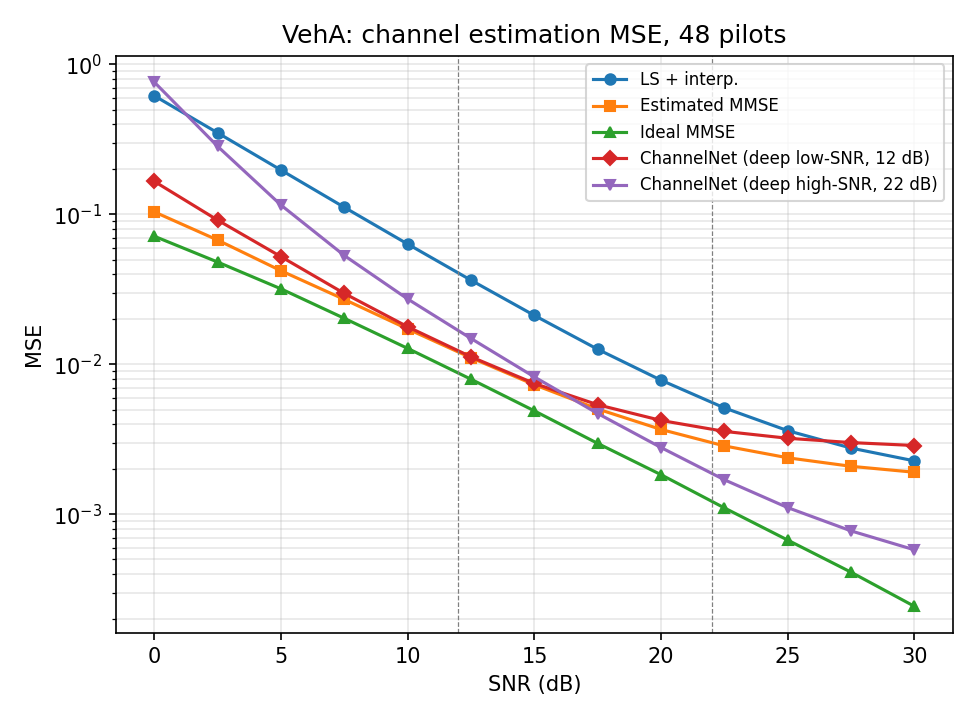
\includegraphics[width=\textwidth]{fig3_VehA_mse_snr.png}\caption{VehA (cf.\ paper Fig.~3)}\end{subfigure}\hfill
    \begin{subfigure}{0.49\textwidth}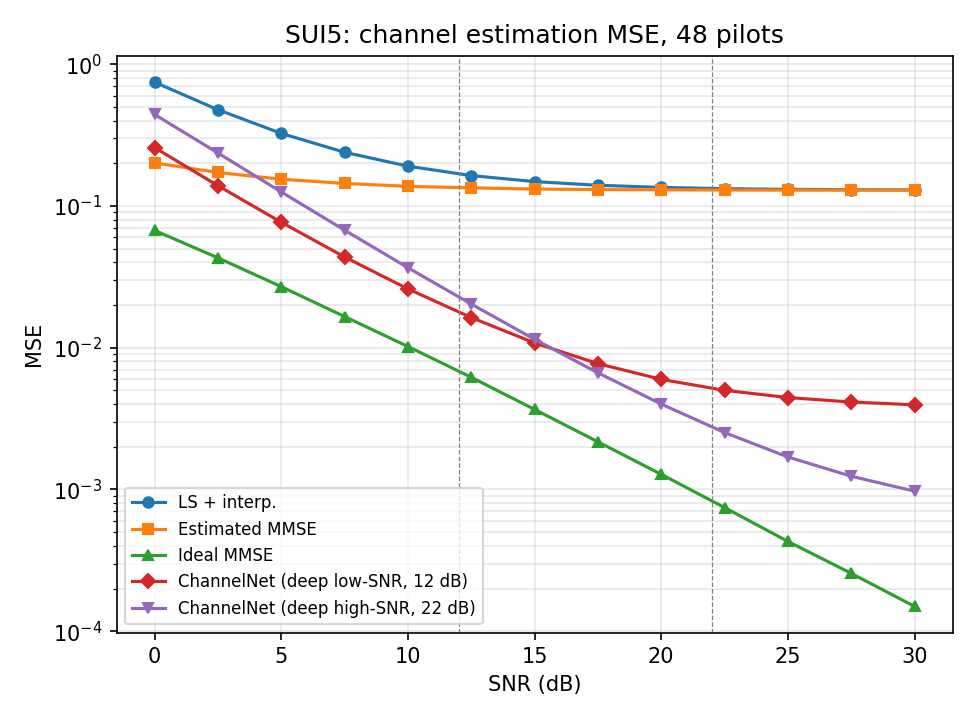
\includegraphics[width=\textwidth]{fig4_SUI5_mse_snr.png}\caption{SUI5 (cf.\ paper Fig.~4)}\end{subfigure}
    \caption{MSE vs.\ SNR, 48 pilots; dashed lines mark the training SNRs}
    \label{fig:fig34}
\end{figure}

\begin{table}[H]
\centering
\caption{Test MSE (complex channel) versus SNR, 48 pilots}
\label{tab:results}
\small
\begin{tabular}{lccccccc}
\toprule
\textbf{Method} & \textbf{0 dB} & \textbf{5 dB} & \textbf{10 dB} & \textbf{15 dB} & \textbf{20 dB} & \textbf{25 dB} & \textbf{30 dB} \\
\midrule
\multicolumn{8}{l}{\textbf{VehA}} \\
LS + interp. & 6.18e-01 & 1.97e-01 & 6.34e-02 & 2.12e-02 & 7.84e-03 & 3.61e-03 & 2.27e-03 \\
Estimated MMSE & 1.04e-01 & 4.21e-02 & 1.72e-02 & 7.31e-03 & 3.68e-03 & 2.38e-03 & 1.91e-03 \\
Ideal MMSE & 7.15e-02 & 3.19e-02 & 1.28e-02 & 4.89e-03 & 1.84e-03 & 6.72e-04 & 2.43e-04 \\
ChannelNet (12 dB) & 1.66e-01 & 5.22e-02 & 1.78e-02 & 7.46e-03 & 4.23e-03 & 3.21e-03 & 2.88e-03 \\
ChannelNet (22 dB) & 7.62e-01 & 1.15e-01 & 2.73e-02 & 8.24e-03 & 2.79e-03 & 1.11e-03 & 5.79e-04 \\
\midrule
\multicolumn{8}{l}{\textbf{SUI5}} \\
LS + interp. & 7.46e-01 & 3.24e-01 & 1.91e-01 & 1.48e-01 & 1.35e-01 & 1.31e-01 & 1.30e-01 \\
Estimated MMSE & 2.01e-01 & 1.54e-01 & 1.37e-01 & 1.31e-01 & 1.30e-01 & 1.29e-01 & 1.29e-01 \\
Ideal MMSE & 6.71e-02 & 2.69e-02 & 1.02e-02 & 3.67e-03 & 1.28e-03 & 4.30e-04 & 1.50e-04 \\
ChannelNet (12 dB) & 2.58e-01 & 7.66e-02 & 2.60e-02 & 1.08e-02 & 5.97e-03 & 4.45e-03 & 3.95e-03 \\
ChannelNet (22 dB) & 4.41e-01 & 1.25e-01 & 3.66e-02 & 1.15e-02 & 4.00e-03 & 1.69e-03 & 9.72e-04 \\
\bottomrule
\end{tabular}
\end{table}

\textbf{VehA.} ChannelNet beats LS everywhere. The 12~dB network is about equal to estimated MMSE below 15~dB. The 22~dB network beats it above about 17~dB: 5.79e-4 vs.\ 1.91e-3 at 30~dB, a $3.3\times$ improvement. Ideal MMSE stays the lower bound, consistent with the paper's finding that ChannelNet is comparable to approximated MMSE on VehA.
\textbf{SUI5.} This is the largest gain. ChannelNet removes the $\approx$0.13 error floor: at 25~dB it reaches 1.69e-3, about \textbf{75$\times$ lower} than LS and estimated MMSE. This agrees with the paper's finding that ChannelNet clearly outperforms ALMMSE on SUI5.

\begin{figure}[H]
    \centering
    \begin{subfigure}{0.49\textwidth}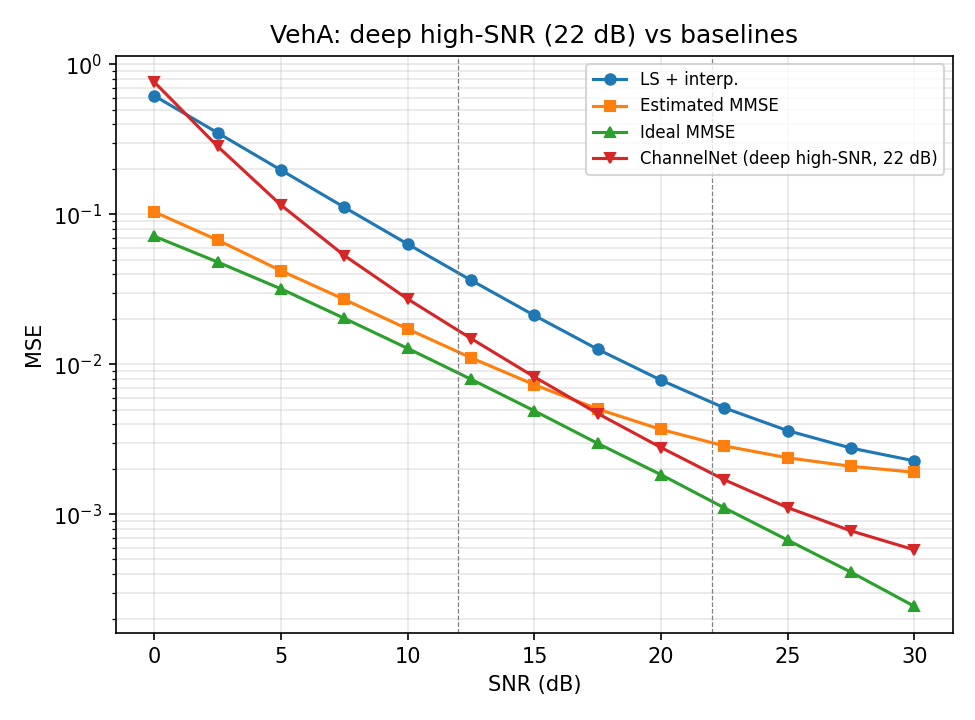
\includegraphics[width=\textwidth]{fig_highsnr_VehA.png}\caption{VehA}\end{subfigure}\hfill
    \begin{subfigure}{0.49\textwidth}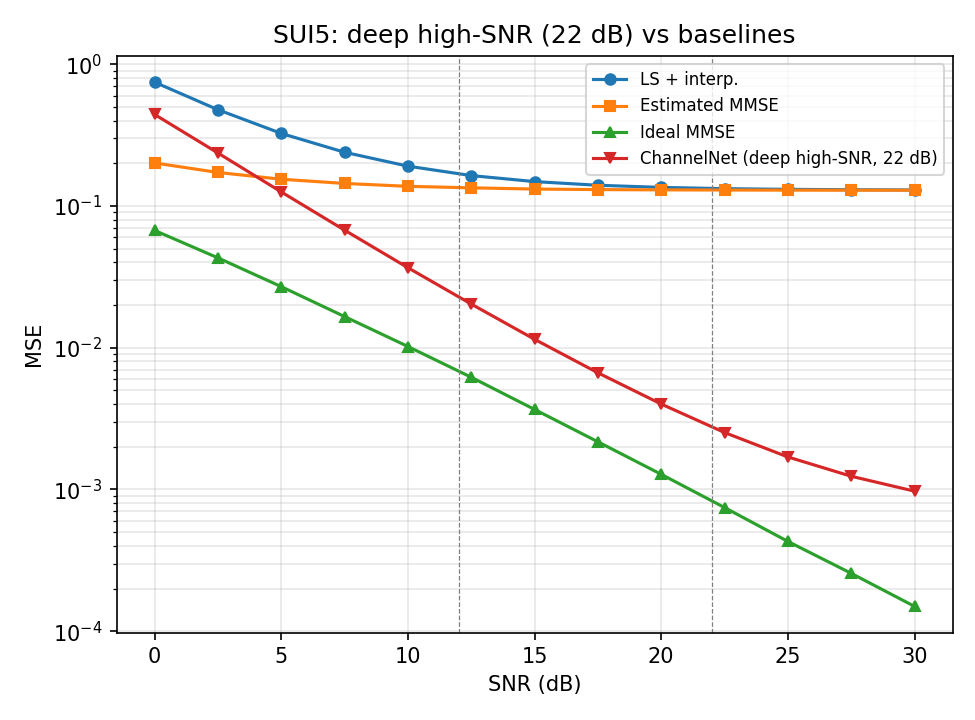
\includegraphics[width=\textwidth]{fig_highsnr_SUI5.png}\caption{SUI5}\end{subfigure}
    \caption{Deep high-SNR case: ChannelNet trained at 22~dB vs.\ LS, estimated and ideal MMSE}
    \label{fig:highsnr}
\end{figure}

\textbf{Deep high-SNR case (Fig.~\ref{fig:highsnr}).} Above about 17~dB, the 22~dB network is the best practical estimator for both channels. At low SNR it collapses: at 0~dB on VehA it gives 0.76, worse than LS at 0.62 (see Section~\ref{sec:discussion}).

\begin{figure}[H]
    \centering
    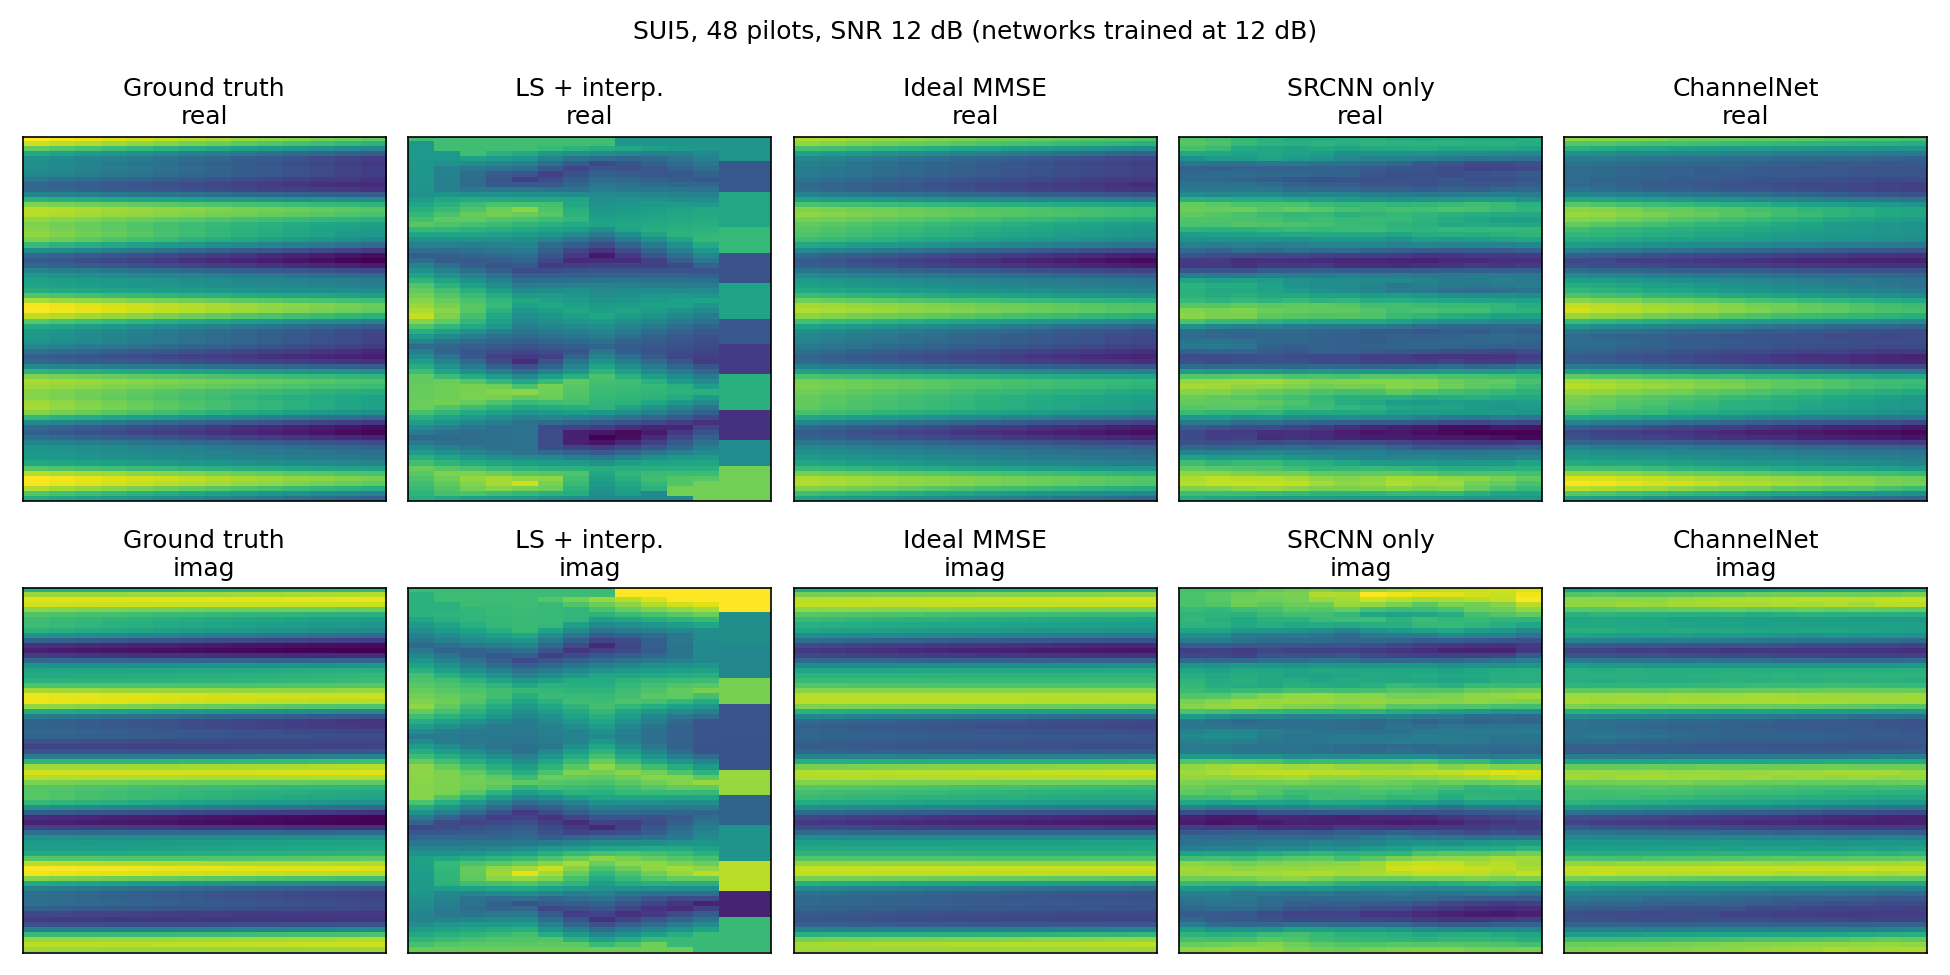
\includegraphics[width=0.92\textwidth]{fig_estimates_SUI5.png}
    \caption{SUI5 test channel at 12~dB: truth, LS + interpolation, ideal MMSE, SRCNN only, ChannelNet}
    \label{fig:est}
\end{figure}

\begin{figure}[H]
    \centering
    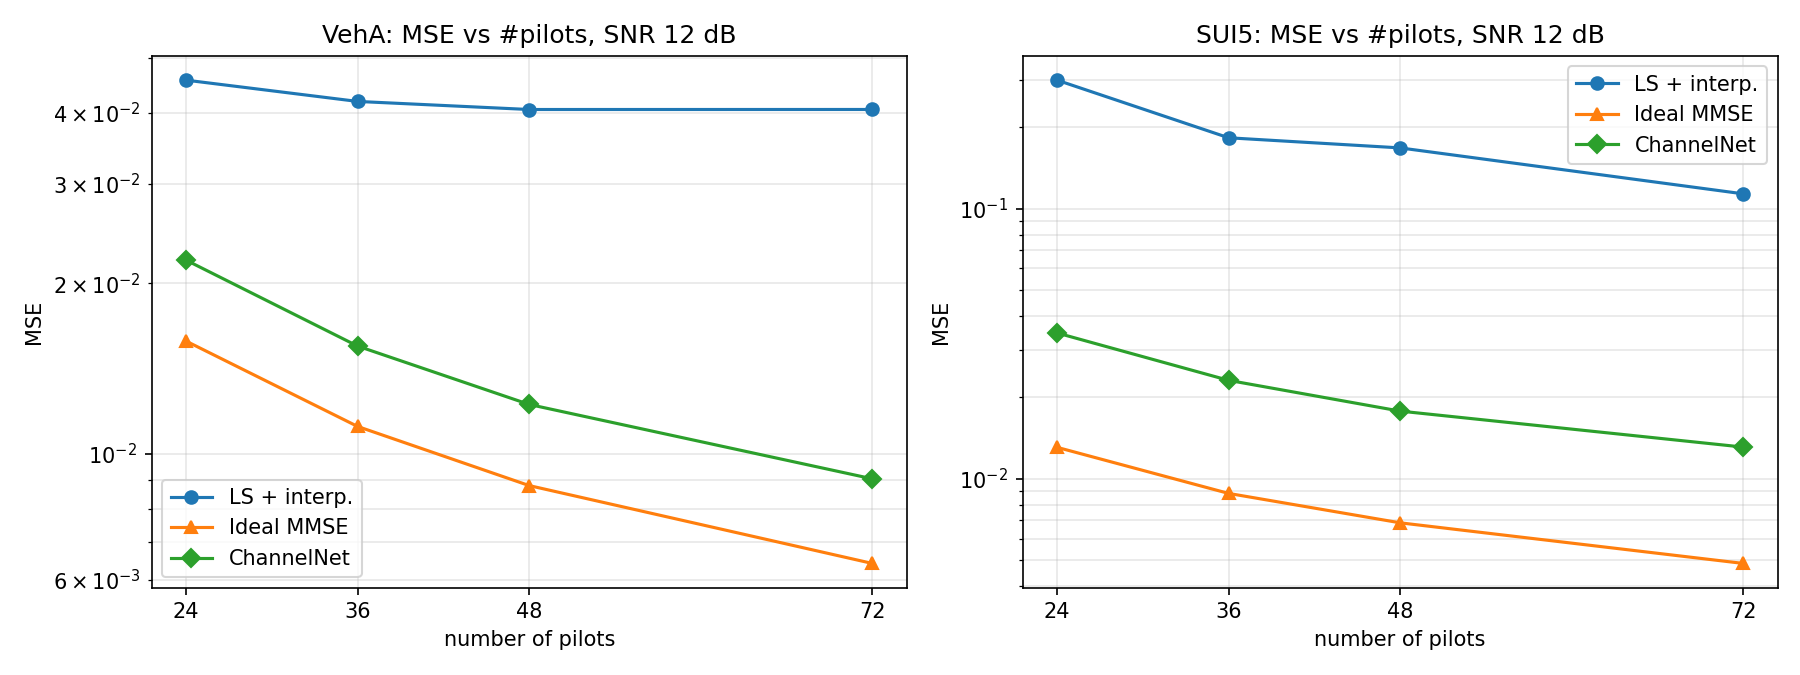
\includegraphics[width=0.78\textwidth]{fig5_mse_pilots.png}
    \caption{MSE vs.\ number of pilots at 12~dB (cf.\ paper Fig.~5); one ChannelNet per pilot count}
    \label{fig:fig5}
\end{figure}

\textbf{Pilot density (Fig.~\ref{fig:fig5}).} ChannelNet improves steadily with more pilots: VehA goes from 2.2e-2 to 9.0e-3, and SUI5 from 3.5e-2 to 1.3e-2, between 24 and 72 pilots. For VehA, LS barely changes, because at 12~dB noise limits it, not pilot spacing. For SUI5, LS improves strongly with density (0.30 $\rightarrow$ 0.11). ChannelNet on SUI5 with 24 pilots is already about $3\times$ better than LS with 72 pilots, so pilot overhead could be reduced. The 24/36/72-pilot networks had at most 20 DnCNN epochs, so their points are slightly pessimistic. Fig.~\ref{fig:est} shows the stages visually: LS leaves blocky artefacts, SRCNN recovers the structure but keeps some noise, and DnCNN removes most of it.

% ============================================================
\section{Discussion: SNR-Specific Training and Generalisation}
\label{sec:discussion}
% ============================================================
\paragraph{Q1. What are the limitations of training at specific SNR values, and how do they affect generalisation?}
Each network is reliable only near the SNR it was trained at (Fig.~\ref{fig:fig34}, Table~\ref{tab:results}):
\begin{packed_enum}
    \item \textbf{High-SNR network at low SNR.} The 22~dB network never saw strong noise. Its denoiser removes only the small residual it learned and passes larger noise through. At 0~dB on VehA it is \emph{worse than LS} (0.76 vs.\ 0.62). On SUI5 it is worse than the 12~dB network up to about 15~dB.
    \item \textbf{Low-SNR network at high SNR.} The 12~dB network learned to smooth heavily. When the noise is small, this smoothing removes real channel detail and causes an error floor. On VehA at 30~dB it is again worse than LS (2.88e-3 vs.\ 2.27e-3); on SUI5 it saturates near 4e-3, while the 22~dB network reaches 9.7e-4.
    \item \textbf{Consequence for deployment.} The two curves cross at about 15--17~dB, so a receiver needs an SNR estimate and several stored networks, or must accept the mismatch loss. Switching between the two networks at 17~dB (\texttt{results/fig\_ablation\_*.png}) always gives the better of the two, but two training points cover 0--30~dB only coarsely. The networks are also specific to one pilot pattern and one channel model, which multiplies the number of models needed.
\end{packed_enum}
Unlike the paper, my high-SNR network does not degrade above about 23~dB; I attribute this to the residual DnCNN formulation and to keeping the best-validation weights.

\paragraph{Q2. How can generalisation across a wider SNR range be improved?}
\begin{packed_enum}
    \item \textbf{Multi-SNR (blind) training:} train one network on frames with SNR drawn over the whole range (e.g.\ 0--30~dB). The blind DnCNN-B model \cite{zhang2017}, trained over a range of noise levels, nearly matches noise-specific models. Curriculum ordering from high to low SNR can help convergence.
    \item \textbf{Noise-level-conditioned networks:} feed $\sigma^2$, or an estimated SNR, as an extra input map, as FFDNet does \cite{zhang2018ffdnet}, so that one network adapts its smoothing to the noise. An OFDM receiver can estimate the SNR easily from pilots or null subcarriers.
    \item \textbf{Bank of networks with SNR switching or blending:} store networks for several SNRs and select or interpolate between them by estimated SNR. This is simple and effective (my switched curve), at the cost of memory.
    \item \textbf{Model-driven / residual designs:} make the noise statistics explicit, for example by unrolling iterative estimators with learned denoisers (LDAMP \cite{he2018}), or use residual networks that refine the LS estimate \cite{li2020reesnet}. These generalise across SNR better than purely black-box mappings.
    \item \textbf{Online adaptation / meta-learning:} fine-tune on a few pilot frames at the current SNR; MAML \cite{finn2017} provides an initialisation suited to fast adaptation.
    \item \textbf{Joint pilot design:} learn the pilot placement together with the estimator \cite{soltani2020pilot,mashhadi2021}, which reduces how much super-resolution the network must perform and hence its sensitivity to noise.
\end{packed_enum}

% ============================================================
\section{Limitations and Conclusion}
% ============================================================
\textbf{Limitations.}
\begin{packed_enum}
    \item SUI5 is a user-defined profile with Jakes Doppler, whereas the standard SUI model uses a rounded Doppler spectrum.
    \item The frequency-domain model (Eq.~\ref{eq:sysmodel}) ignores ICI and ISI, even though SUI5's 10~$\mu$s path exceeds the 4.7~$\mu$s cyclic prefix.
    \item Ideal MMSE is an unrealisable lower bound, not a practical competitor.
    \item Each training frame uses one fixed noise realisation, as in the paper.
    \item One network is needed per SNR, pilot pattern and channel model, and DnCNN (667k parameters) is much more costly at inference than LS or a precomputed MMSE matrix.
\end{packed_enum}

\textbf{Conclusion.} I reproduced ChannelNet end to end. On VehA, it matches practical MMSE at low SNR and beats it at high SNR. On the highly frequency-selective SUI5 channel, it removes the interpolation error floor of LS and estimated MMSE, with up to two orders of magnitude lower MSE. Its main weakness is SNR specificity, and multi-SNR or noise-conditioned training is the most direct remedy.

{\small
\begin{thebibliography}{99}

\bibitem{soltani2019}
M. Soltani, V. Pourahmadi, A. Mirzaei, and H. Sheikhzadeh,
``Deep Learning-Based Channel Estimation,''
\textit{IEEE Communications Letters}, vol. 23, no. 4, pp. 652--655, Apr. 2019.

\bibitem{dong2016}
C. Dong, C. C. Loy, K. He, and X. Tang,
``Image Super-Resolution Using Deep Convolutional Networks,''
\textit{IEEE Trans. Pattern Analysis and Machine Intelligence}, vol. 38, no. 2, pp. 295--307, 2016.

\bibitem{zhang2017}
K. Zhang, W. Zuo, Y. Chen, D. Meng, and L. Zhang,
``Beyond a Gaussian Denoiser: Residual Learning of Deep CNN for Image Denoising,''
\textit{IEEE Trans. Image Processing}, vol. 26, no. 7, pp. 3142--3155, 2017.

\bibitem{vienna}
S. Pratschner, B. Tahir, L. Marijanovic, M. Mussbah, K. Kirev, R. Nissel, S. Schwarz, and M. Rupp,
``Versatile Mobile Communications Simulation: The Vienna 5G Link Level Simulator,''
\textit{EURASIP Journal on Wireless Communications and Networking}, 2018:226, 2018.

\bibitem{edfors1998}
O. Edfors, M. Sandell, J.-J. van de Beek, S. K. Wilson, and P. O. B\"orjesson,
``OFDM Channel Estimation by Singular Value Decomposition,''
\textit{IEEE Trans. Communications}, vol. 46, no. 7, pp. 931--939, 1998.

\bibitem{zhang2018ffdnet}
K. Zhang, W. Zuo, and L. Zhang,
``FFDNet: Toward a Fast and Flexible Solution for CNN-Based Image Denoising,''
\textit{IEEE Trans. Image Processing}, vol. 27, no. 9, pp. 4608--4622, 2018.

\bibitem{he2018}
H. He, C.-K. Wen, S. Jin, and G. Y. Li,
``Deep Learning-Based Channel Estimation for Beamspace mmWave Massive MIMO Systems,''
\textit{IEEE Wireless Communications Letters}, vol. 7, no. 5, pp. 852--855, 2018.

\bibitem{li2020reesnet}
L. Li, H. Chen, H.-H. Chen, and Y. Liu,
``Deep Residual Learning Meets OFDM Channel Estimation,''
\textit{IEEE Wireless Communications Letters}, vol. 9, no. 5, pp. 615--618, 2020.

\bibitem{finn2017}
C. Finn, P. Abbeel, and S. Levine,
``Model-Agnostic Meta-Learning for Fast Adaptation of Deep Networks,''
in \textit{Proc. ICML}, 2017, pp. 1126--1135.

\bibitem{soltani2020pilot}
M. Soltani, V. Pourahmadi, and H. Sheikhzadeh,
``Pilot Pattern Design for Deep Learning-Based Channel Estimation in OFDM Systems,''
\textit{IEEE Wireless Communications Letters}, vol. 9, no. 12, pp. 2173--2176, 2020.

\bibitem{mashhadi2021}
M. B. Mashhadi and D. G\"und\"uz,
``Pruning the Pilots: Deep Learning-Based Pilot Design and Channel Estimation for MIMO-OFDM Systems,''
\textit{IEEE Trans. Wireless Communications}, vol. 20, no. 10, pp. 6315--6328, 2021.

\bibitem{github}
Dhavala.H,
``IMT2023579-COM-837-ML-for-Wireless-Communication,''
GitHub repository.
[Online]. Available: \url{https://github.com/DHardhik/IMT2023579-COM-837-ML-for-Wireless-Communication}

\end{thebibliography}
}

\end{document}
